\chapter{Tecnologie e piattaforme}\label{cap:2}
In questo capitolo verranno trattate le tecnologie utilizzate, a partire dai linguaggi, i tools utilizzate e le piattaforme hardware di lavoro. È stato fondamentale l’utilizzo di macchine in remoto per eseguire le operazioni di training del modello. In questo caso le macchine messe a disposizione dall’Università Parthenope e dal CNR sono state fondamentali in quanto hanno garantito stabilità ed efficienza.

\section{Linguaggi e tools}\label{sec:2.1}
La scelta del linguaggio di programmazione è stata importante in quanto ci sono tantissimi linguaggi con librerie adatte allo scopo, solo pochi ricevono costante supporto e sono anche utilizzati nel mondo del lavoro.

\subsection{Python}\label{sec:2.1.1}
\textbf{Python} è un linguaggio di programmazione dinamico orientato agli oggetti utilizzabile per molti tipi  di sviluppo software. Offre un forte supporto all'integrazione con altri linguaggi e programmi, è fornito di una estesa libreria standard e può essere imparato in pochi giorni. Python inoltre è fornito delle librerie di bioinformatica adatte allo scopo del software realizzato. Di seguito le principali utilizzate:

\begin{itemize}
    \item \textbf{pubchempy}, per le ricerche chimiche per nome, sottostruttura e somiglianza, standardizzazione chimica, conversione tra formati di file chimici, rappresentazione e recupero delle proprietà chimiche
    \item \textbf{prody}, per l'analisi della dinamica strutturale delle proteine
    \item \textbf{pandas}, per la manipolazione ed analisi dei dati
    \item \textbf{Tkinter/customTkinter}, per la realizzazione dell'interfaccia grafica
    \item \textbf{MolKit}, pacchetto che fornisce classi per leggere le molecole in diversi formati di file (PDB, Mol2...) e costruire una struttura gerarchica ad albero che riproduce la struttura interna della molecola
    \item \textbf{Matplotlib}, per la creazione di visualizzazioni statiche, animate e interattive
    \item \textbf{customTkinter}, per la realizzazione dell'interfaccia grafica
    \item \textbf{numpy}, per la gestione delle strutture dati
    \item \textbf{os}, per la gestione dei files
\end{itemize} 

La versione di Python utilizzata è la \textbf{2.7} in quanto maggiormente compatibile con le librerie e i pacchetti utilizzati.

\subsection{ADFRsuite}\label{sec:2.1.2}
\textbf{AutoDockFR} (o \textbf{ADFR} in breve) è un programma per il \textbf{docking tra proteine e ligandi} sviluppato nel laboratorio Sanner dello Scripps Research sotto l'egida di \textit{AutoDock}.\newline
Utilizza:

\begin{itemize}
    \item la funzione di scoring di \textit{AutoDock4}, implementata in una libreria C++ ed inglobata in Python
    \item un proprio algoritmo genetico in grado di evolvere e ottimizzare più soluzioni simultaneamente, di gestire un gran numero di legami ruotabili e di terminare le iterazioni al momento della convergenza, cioè potenzialmente senza esaurire il numero assegnato di valutazioni della funzione energia
    \item una rappresentazione generica di flessibilità molecolare, chiamata \textit{Albero di Flessibilità}, che consente di incorporare una varietà di movimenti molecolari sia nel ligando che nel recettore.
\end{itemize}

Pur supportando le modalità di docking disponibili in \textit{AutoDock4} e \textit{Vina}, è stato progettato specificamente per includere la \textbf{flessibilità del recettore} e supporta anche il \textbf{docking covalente}. Il suo algoritmo genetico personalizzato consente il docking di ligandi con più legami ruotabili rispetto ad \textit{AutoDock4}.\newline
Viene distribuito come parte della suite del software \textit{ADFR}, che fornisce strumenti aggiuntivi per facilitare il docking automatizzato.\newline
\textit{ADFR} implementa diverse caratteristiche che aiutano a semplificare la procedura di docking e a supportare la gestione e la riproducibilità degli esperimenti di docking attraverso la prova dei dati. Vengono utilizzati file autodocumentati per memorizzare: 

\begin{itemize}
    \item la rappresentazione del sito di binding (cioè \textbf{i file .trg target})
    \item i risultati del docking (file \textbf{.dro Docking Results Object})
    \item I metadati memorizzati in questi file non solo supportano la riproducibilità, ma riducono anche i rischi di errori dell'operatore.
\end{itemize}

ADFR legge i \textbf{ligandi} preparati per il docking con AutoDock, cioè nel formato PDBQT e organizza la flessibilità del ligando in base ai legami ruotabili. Un file PDBQT può essere generato da un file \textit{.pdb} di un ligando utilizzando il comando \textit{prepar\_ligand}.  Il \textbf{recettore} è specificato come file target, cioè un singolo file che descrive il recettore. I file target possono essere calcolati per un recettore nel formato PDBQT dal comando utilizzando il programma \textit{\textbf{agfr}} o l'interfaccia grafica \textit{\textbf{agfrgui}}. Un file PDBQT può essere generato da un file pdb di un recettore utilizzando il comando \textit{prepare\_receptor} della suite \textit{ADFR}. \newline
\textit{ADFR} è implementato nei moderni linguaggi di programmazione orientati agli oggetti e si basa su componenti software riutilizzabili. I componenti critici per le prestazioni sono implementati in C e C++ (ad esempio ADFRcc), mentre altri sono implementati in Python (ADFR, AutoSite, MolKit2, prody). \textit{ADFR} è rilasciato sotto la licenza open source LGPL v2.\newline 
In particolare per l'applicazione trattata sono stati utilizzati i due script: \textbf{prepare\_ligand4} e \textbf{prepare\_receptors4}, rispettivamente per la preparazione dei ligandi e dei recettori e per effettuare la loro conversione dal formato \textit{.pdb} al formato \textit{.pdbqt} necessario per la procedura di docking.

\subsection{MGLTools}\label{sec:2.1.3}
La suite software \textbf{MGLTools} è stata sviluppata nel laboratorio Sanner presso il Center for Computational Structural Biology (CCRB) precedentemente noto come Molecular Graphics Laboratory (MGL) dello Scripps Research Institute per la visualizzazione e l'analisi delle strutture molecolari. MGLTools comprende:

\begin{itemize}
    \item \textbf{Python Molecular Viewer (PMV)}, un visualizzatore molecolare di uso generale
    \item \textbf{AutoDockTools (ADT)}, un insieme di comandi PMV sviluppati specificamente per supportare gli utenti di AutoDock
    \item \textbf{Vision}, un ambiente di programmazione visuale.
\end{itemize}

Questi strumenti software sono altamente integrati e basati su componenti software riutilizzabili implementati in Python e C++ (con binding Python). Il kit di strumenti grafici sottostante è Tk (Tkinter).L'ultima versione di MGLtools è la 1.5.7 che fornisce:

\begin{itemize}
    \item un widget della dashboard ridisegnato
    \item un widget per la visualizzazione delle sequenze
    \item ottimizzazioni delle prestazioni
    \item nuovi comandi per i calcoli di sovrapposizione e RMSD
\end{itemize}

\subsection{Open Babel}\label{sec:2.1.4}
\textbf{Open Babel} è un tool per applicazioni di chimica progettato per interpretare i molteplici formati dei dati chimici e per cercare, convertire, analizzare o archiviare dati da modellistica molecolare, chimica, materiali a stato solido, biochimica o aree correlate.\newline
La versione di OpenBabel 2.3 converte fino a 110 formati di file chimici.\newline
I database sono ampiamente utilizzati per memorizzare le informazioni chimiche soprattutto nell'industria farmaceutica. Un requisito fondamentale di un database di questo tipo è la capacità di indicizzare le strutture strutture chimiche in modo che possano essere recuperate rapidamente, data una quary di ricerca. Open Babel offre questa funzionalità utilizzando un'indicizzazione basata sul percorso. Questa indicizzazione, FP2 in Open Babel, identifica tutte le sottostrutture lineari e ad anello della molecola di lunghezza da 1 a 7 (escluse le sottostrutture a 1 atomo C e N) e le mappa in una stringa di bit di lunghezza su una stringa di bit di lunghezza 1024 utilizzando una funzione di hash. Se una molecola interrogata è una sottostruttura di una molecola di destinazione, tutti i bit molecola di destinazione, allora tutti i bit impostati nella molecola di query saranno impostati anche nella molecola di destinazione. Le indicizzazioni
di due molecole possono anche essere utilizzate per calcolare la somiglianza strutturale utilizzando il coefficiente di Tanimoto, il numero di bit in comune diviso per tutti i bit dell'insieme.
Chiaramente, la ricerca iterativa dello stesso insieme di molecole comporterà l'uso ripetuto dello stesso insieme di indicizzazioni. Per evitare la necessità di ricalcolare le indicizzazioni per un particolare file multi-molecola (come un file SDF), Open Babel fornisce un formato fastindex che memorizza esclusivamente un'indicizzazione insieme a un indice nel file originale. Questo indice porta a un rapido aumento della velocità di ricerca di corrispondenze a a fronte di una quary: insiemi di dati con diversi milioni di molecole sono facilmente consultabili in modo interattivo. In questo in questo modo, un file multi-molecola può essere utilizzato come un'alternativa efficace a un sistema di database chimico\cite{o2011open}.

\section{Database}\label{sec:2.2}
\textbf{PubChem} è il più grande database al mondo di informazioni chimiche liberamente accessibili, attraverso il quale è possibile cercare le sostanze chimiche per nome, formula molecolare, struttura e altri identificatori. Inoltre è possibile trovare proprietà chimiche e fisiche, attività biologiche, informazioni sulla sicurezza e sulla tossicità, brevetti, citazioni bibliografiche e altro ancora. L'interfaccia tra l'applicazione ed il database è realizzata mediante la libreria di Python \textbf{pubchempy}.\newline
PubChem è un database di molecole chimiche, gestito dal centro nazionale per l'Informazione biotecnologica statunitense (NCBI), parte della biblioteca nazionale di medicina (NLM) dell'istituto nazionale della sanità americano (NIH). L'accesso al database PubChem può essere eseguito liberamente attraverso un sito web e possono essere scaricati dati riguardanti milioni di strutture di composti e dati descrittivi tramite il protocollo FTP.PubChem possiede descrizioni di molecole con meno di 1000 atomi e 1000 legami. \newline 
PubChem gestisce i dati in tre database interconnessi: \textbf{Substance, Compound e BioAssay}. Il database Substance archivia le descrizioni delle sostanze chimiche fornite dai depositanti. Il database Compound archivia le strutture chimiche uniche estratte dal database Substance attraverso la standardizzazione delle strutture. Il database BioAssay contiene la descrizione e i risultati degli esperimenti di analisi biologica.

\section{Autodock}\label{sec:2.3}
\textbf{AutoDock} è un programma di docking che utilizza un algoritmo genetico, il \textit{Lamarckian Genetic Algorithm}, per il calcolo della pose migliore che interagisce con il sito attivo della proteina. Dopo aver calcolato inizialmente una popolazione di possibili soluzioni, l’algoritmo ne selezionerà una parte in base alle funzioni di scoring e darà origine a una nuova popolazione di soluzioni figlie, da cui avrà inizio un secondo ciclo di generazione e così via. In questo modo il “genotipo”, ovvero la stringa binaria a cui corrisponde ciascun ligando, verrà influenzato da fattori esterni, esattamente come nell’ipotesi lamarckiana.\newline
Le popolazioni di soluzioni sono ottenute tramite operatori genetici (mutazioni, crossover e migrazioni) che imitano quelli biologici. I gradi di libertà sono codificati in geni o stringhe binarie, e a geni e cromosomi è assegnato un valore basato sulla fitness della scoring function. Le operazioni di mutazione causano cambiamenti nel valore di un gene, mentre il crossover muove un set di geni da un cromosoma “genitore” ad un altro; la migrazione invece muove singoli geni da una sottopopolazione ad un’altra.\newline
L’interazione tra ligando e recettore è valutata in due fasi, calcolando la variazione di energia intramolecolare del passaggio dalla forma libera a quella legata e la variazione di energia libera intermolecolare implicata nello stesso passaggio.\newline
Per effettuare il docking è necessario per prima cosa preparare le coordinate di ligando e recettore. La preparazione delle coordinate è la fase più importante nella procedura, poiché in esse sono inclusi parametri fondamentali come: idrogeni polari, atom – type e cariche parziali. Le coordinate del ligando originale e della macromolecola sono trattate separatamente ed i loro file sono in un formato particolare, il PDBQT.

\section{Autodock Vina}\label{sec:2.4}
\textbf{AutoDock Vina} è  un nuovo programma per il docking molecolare e lo screening virtuale. Vina rappresenta la nuova versione di AutoDock, ed infatti presenta molte similitudini con il suo predecessore ma, allo stesso tempo, anche molte differenze. Una differenza importante consiste nella velocità di calcolo, dato che Vina è molto poco dispendioso sotto questo punto di vista; altra differenza fondamentale è rappresentata dal fatto che al momento del calcolo della griglia, Vina calcola internamente ed automaticamente le “grid maps” impiegate in AutoDock. Questo costituisce un grande vantaggio in termini di facilità e velocità di esecuzione. Inoltre, le funzioni di scoring e gli algoritmi utilizzati in questo tipo di analisi risultano essere completamente diversi rispetto al suo predecessore, cosa che porta a considerare Vina quasi come un software a sé stante. Vina migliora al tempo stesso in modo significativo l'accuratezza delle previsioni delle modalità di legame. Un'ulteriore miglioramento è ottenuta grazie al parallelismo, che utilizza il multithreading su macchine multicore. AutoDock Vina calcola automaticamente le mappe della griglia e raggruppa i risultati in modo trasparente per l'utente. Autodock vina all'interno del software prende in input i ligandi ed i recettori in formato \textit{.pdbqt}.

\subsection{Funzione di scoring}\label{sec:2.4.1}
La funzione di scoring di AutoDock Vina (qui indicata come Vina) può essere rappresentata attraverso la seguente formula:

\begin{equation}
    c = \sum_{i<j}f_{t_it_j}(r_{ij})
\end{equation}

dove la sommatoria è su tutte le coppie di atomi che possono muoversi l'uno rispetto all'altro, escludendo normalmente le interazioni 1-4, ovvero gli atomi separati da tre legami covalenti consecutivi. Ad ogni atomo $i$ viene assegnato un tipo $t_i$ e un insieme simmetrico di funzioni di interazione $f_{t_it_j}$ della distanza interatomica $r_{ij}$ da definire.\newline
Questo valore può essere visto come una somma di contributi intermolecolari e intramolecolari:

\begin{equation}
    c = c_{inter} + c_{intra}
\end{equation}

L'algoritmo di ottimizzazione, descritto in seguito, cerca di trovare il minimo globale di $c$ e di altre conformazioni a basso punteggio, che poi classifica.\newline 
L'energia libera di legame prevista viene calcolata a partire dalla parte intermolecolare della conformazione con il punteggio più basso, designata come:

\begin{equation}
    s_1 = g(c_1 - c_{intra1}) = g(c_{inter1})
\end{equation}

dove la funzione $g$ può essere una funzione arbitraria strettamente crescente possibilmente non lineare.\newline Nell'output le altre conformazioni a basso punteggio vengono formalmente restituite dai valori di $s$, ma per preservare il ranking, si utilizza $c_{intra}$ come migliore modalità di legame:

\begin{equation}
    s_i = g(c_i - c_{intra1})
\end{equation}

Per ragioni di modularità, gran parte del programma non fa riferimento ad alcuna forma funzionale delle interazioni $f_{t_it_j}$ o $g$. Essenzialmente, queste funzioni vengono passate come parametro per il resto del codice. Inoltre, il programma è stato progettato in modo tale da poter utilizzare schemi di tipizzazione degli atomi come la tipizzazione degli atomi di AutoDock4 o SYBIL.\newline

\begin{table}[H]
    \centering
    \begin{tabular}{|l|l|}
        \hline
        \textbf{Pesi} & \textbf{Termini}\\
        \hline
        $-0.0356$ & $gauss_1$\\
        $-0.00516$ & $gauss_2$\\
        $0.840$ & $repulsion$\\
        $-0.0351$ & $hydrophobic$\\
        $-0.587$ & $hydrogen bonding$\\
        $0.0585$ & $N_{rot}$\\
        \hline
    \end{tabular}
    \caption{Funzione di scoring pesi e termini}
    \label{tab:Tabella Pesi e Termini}
\end{table}

La particolare implementazione della funzione di scoring che verrà presentata è stata ispirata principalmente da X-score e come tale è stato messo a punto utilizzando PDBbind. Tuttavia, alcuni termini sono diversi da X-score e, nel mettere a punto la funzione di scoring, si è andati oltre la regressione lineare. Inoltre, va notato che Vina classifica le conformazioni secondo l'eq. (2.2) o, equivalentemente, eq. (2.4), mentre X-score conta solo i contributi intermolecolari.
Per quanto ne sappiamo, X-score non è stato implementato in un programma di docking, ignorare i vincoli interni potrebbe portare l'algoritmo di ottimizzazione a ricercare strutture corrotte all'interno.\newline
La derivazione della nostra funzione di scoring combina alcuni vantaggi tra quelli potenzialmente conosciuti e le funzioni di scoring empiriche: estrae informazioni empiriche da entrambe le preferenze conformazionali del sia dei complessi recettore-ligando sia dalle misure sperimentali affini.\newline 
Lo schema di tipizzazione degli atomi segue quello di X-score. Gli atomi di idrogeno non sono considerati esplicitamente, se non per la tipizzazione degli atomi, e sono omessi dall'eq. (2.1).\newline
Le funzioni di interazione $f_{t_it_j}$ sono definite rispetto alla distanza di superficie  $d_{ij} = r_{ij} - R_{ti} - Rtj$:

\begin{equation}
    f_{t_it_j}(r_{ij}) \equiv h_{t_it_j}(d_{ij})
\end{equation}

dove $R_t$ è il raggio di van der Waals dell'atomo di tipo $t$.\newline
Nella nostra funzione di scoring, $h_{t_it_j}$ è una somma ponderata di interazioni steriche (i primi tre termini nella tabella 2.1), identica per tutte le coppie di atomi, interazione idrofobiche tra atomi idrofobici e, dove possibile, legami a idrogeno. I pesi sono mostrati nella tabella 2.1. I termini sterici sono i seguenti:

\begin{equation}
    gauss_1(d)=e^{-(d/0.5\mathring{A})^2}
\end{equation}

\begin{equation}
    gauss_2(d)=e^{-((d/0.5\mathring{A})/2\mathring{A})^2}
\end{equation}

\begin{equation}
    repulsion(d) = \begin{cases}
                        d^2, se & d < 0\\
                        0, se & d \geq 0
                    \end{cases}
\end{equation}

Il termine idrofobico è uguale a $1$, quando $d < 0,5\mathring{A}$; $0$, quando $d > 1,5\mathring{A}$, ed è interpolato linearmente tra questi valori. Il termine di legame a idrogeno è uguale a $1$, quando $d < -0,7\mathring{A}$; $0$, quando $d < 0,5\mathring{A}$, e viene interpolato linearmente tra questi valori. Seguendo Xscore, trattiamo formalmente i metalli come donatori di legami a idrogeno. In questa in questa implementazione, tutte le funzioni di interazione $ f_{t_it_j}$ sono tagliate a $r_{ij} = 8\mathring{A}$.\newline
La Figura 1 mostra i termini sterici ponderati da soli o combinati con i termini idrofobici o H
con le interazioni idrofobiche o di legame H\cite{trott2010autodock}.

\begin{figure}[H]
    \centering
    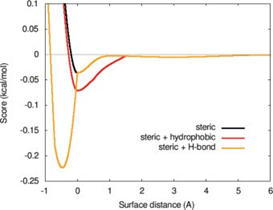
\includegraphics{immagini/funzioneScoringPesata.png}
    \caption{Funzione di scoring pesata}
    \label{fig:Funzione di scoring pesata}
\end{figure}
